\documentclass{beamer}

\mode<presentation>{
	\usetheme{CambridgeUS}
	\usecolortheme{crane}
	\usefonttheme{default}
}

\usepackage{graphicx}
\usepackage{booktabs}
\usepackage{ragged2e}
\usepackage[export]{adjustbox}
\usepackage{minted}
\usemintedstyle{monokai}

\usepackage{aut}

%----------------------------------------------------------------------------------------
%	TITLE PAGE
%----------------------------------------------------------------------------------------
\title[Introduction to KAA Platform]{KAA Platform}
\author{IoT Lab @ AUT}
\institute[]{Amirkabir University of Technology}
\date{\today}
\titlegraphic{\hspace*{5cm}
\includegraphics[width=2cm]{figs/aut_logo.jpeg}}

\begin{document}

\begin{frame}
\titlepage
\end{frame}

%----------------------------------------------------------------------------------------
%	PRESENTATION SLIDES
%----------------------------------------------------------------------------------------

%------------------------------------------------
\begin{frame}
	\frametitle{Outline}
	\begin{itemize}
		\item What is Kaa ?
		\item Where is Kaa ?
		\item What does Kaa do for us ?
	\end{itemize}
\end{frame}

%------------------------------------------------
\begin{frame}
	\frametitle{Outline}
	\begin{itemize}
		\item What is Kaa ?
		\item \textcolor{LightGray}{Where is Kaa ?}
		\item \textcolor{LightGray}{What does Kaa do for us ?}
	\end{itemize}
\end{frame}

%------------------------------------------------
\begin{frame}
	\frametitle{Kaa ?!}
	\begin{block}{
		\centering\textcolor{darkred}{What is Kaa\ldots}}
		\justifying
		[Kaa]: 100\% open-source Internet of Things middleware platform for everyone.
	\end{block}
	\begin{block}{
		\centering\textcolor{darkred}{What is Kaa\ldots}}
		\justifying
		[Wikipedia]: Kaa is a fictional character that Rudyard Kipling describes him as
		an exceptionally long, yellowish Indian rock python.
	\end{block}
	\centering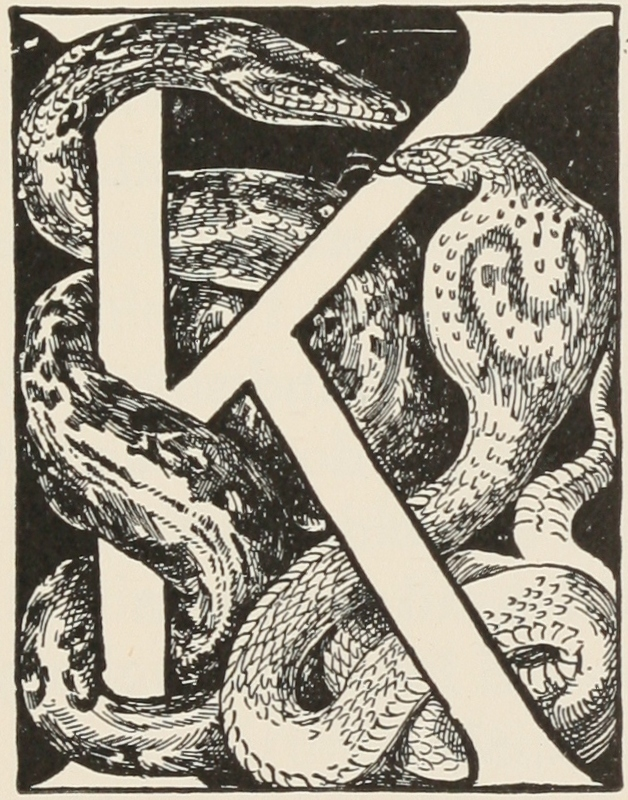
\includegraphics[width=3cm]{figs/kaa.jpeg}
\end{frame}

%------------------------------------------------
\begin{frame}
	\frametitle{What is Kaa ?}
	\centering Kaa is a middleware platform for rapid creation of IoT solutions.
	\vspace{1cm}
	\begin{itemize}
		\item Reliable foundation for developing your connected products.
		\item \textcolor{TextGreen}{Transport-agnostic} link between the hardware and application worlds.
		\item Much more than just a message bus.
		\item \textcolor{TextOrange}{Customizable} middleware that implements necessary functional patterns for the IoT.
		\item \textcolor{Ocean}{Cloud enablement} software for your hardware products.
	\end{itemize}
\end{frame}

%------------------------------------------------
\begin{frame}
	\frametitle{What is Kaa ?}
	\centering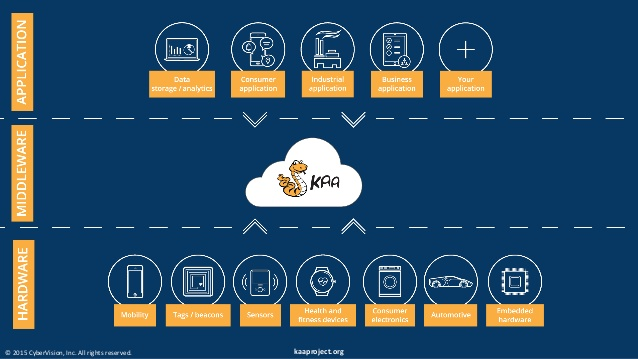
\includegraphics[width=10cm]{diags/kaa-arch-1.jpg}
\end{frame}

%------------------------------------------------
\begin{frame}
	\frametitle{Outline}
	\begin{itemize}
		\item \textcolor{LightGray}{What is Kaa ?}
		\item Where is Kaa ?
		\item \textcolor{LightGray}{What does Kaa do for us ?}
	\end{itemize}
\end{frame}

%------------------------------------------------
\begin{frame}
	\frametitle{Thing Side}
	\centering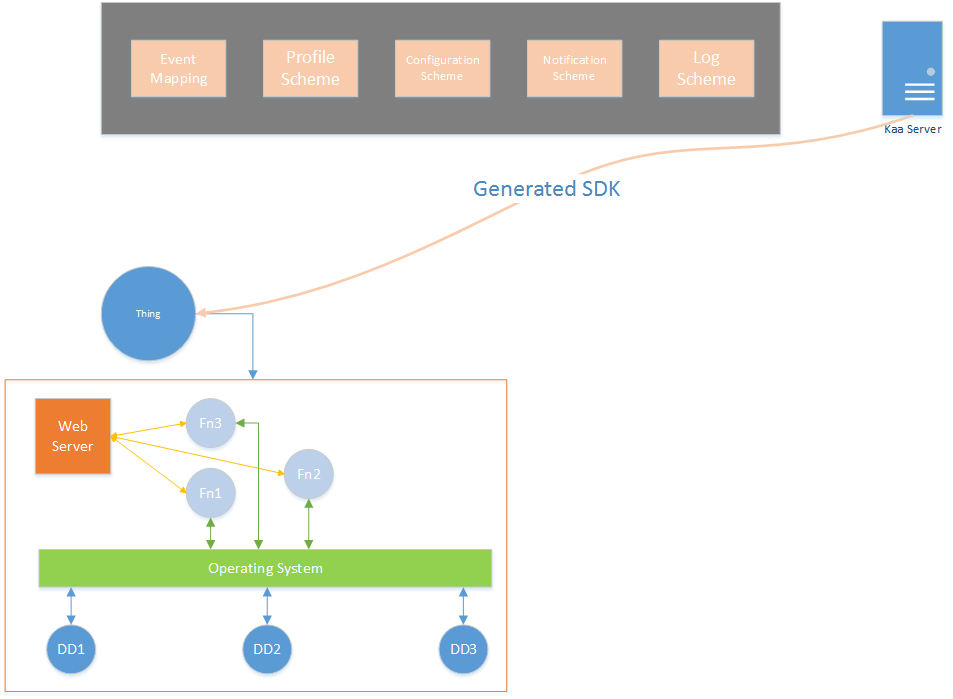
\includegraphics[width=10cm]{diags/kaa-arch-2.png}
\end{frame}

\end{document}
